\documentclass[11pt,letterpaper]{article}

\usepackage[spanish]{babel}
\usepackage[utf8]{inputenc}
\usepackage[T1]{fontenc}
\usepackage{lmodern}
\usepackage{geometry}
\usepackage{graphicx}
\usepackage{booktabs}
\usepackage{longtable}
\usepackage{array}
\usepackage{float}
\usepackage{xcolor}
\usepackage{hyperref}
\usepackage{caption}
\usepackage{enumitem}
\usepackage{fancyhdr}
\usepackage{titlesec}

\geometry{margin=2.35cm}
\setlength{\parskip}{0.65em}
\setlength{\parindent}{0pt}
\hypersetup{
    colorlinks=true,
    linkcolor=black,
    urlcolor=cobreoscuro,
    citecolor=black
}

\definecolor{cobre}{HTML}{B55A2A}
\definecolor{cobreoscuro}{HTML}{6B331B}
\definecolor{mineral}{HTML}{182027}
\definecolor{gris}{HTML}{555555}

\pagestyle{fancy}
\fancyhf{}
\lhead{\textcolor{gris}{Tarea 1}}
\rhead{\textcolor{gris}{Minería chilena}}
\cfoot{\thepage}

\titleformat{\section}{\Large\bfseries\color{cobreoscuro}}{\thesection}{0.8em}{}
\titleformat{\subsection}{\large\bfseries\color{mineral}}{\thesubsection}{0.8em}{}
\titleformat{\subsubsection}{\normalsize\bfseries\color{cobreoscuro}}{\thesubsubsection}{0.8em}{}
\newcommand{\code}[1]{\texttt{\detokenize{#1}}}

\title{
    \vspace{-1.2cm}
    \textbf{\Huge Producción mensual de cobre de mina en Chile}\\[0.25cm]
    \Large Análisis exploratorio, preprocesamiento, visualización y limpieza de datos
}
\author{Ciencia de Datos para Economía y Gestión}
\date{Tarea 1}

\begin{document}
\maketitle

\begin{center}
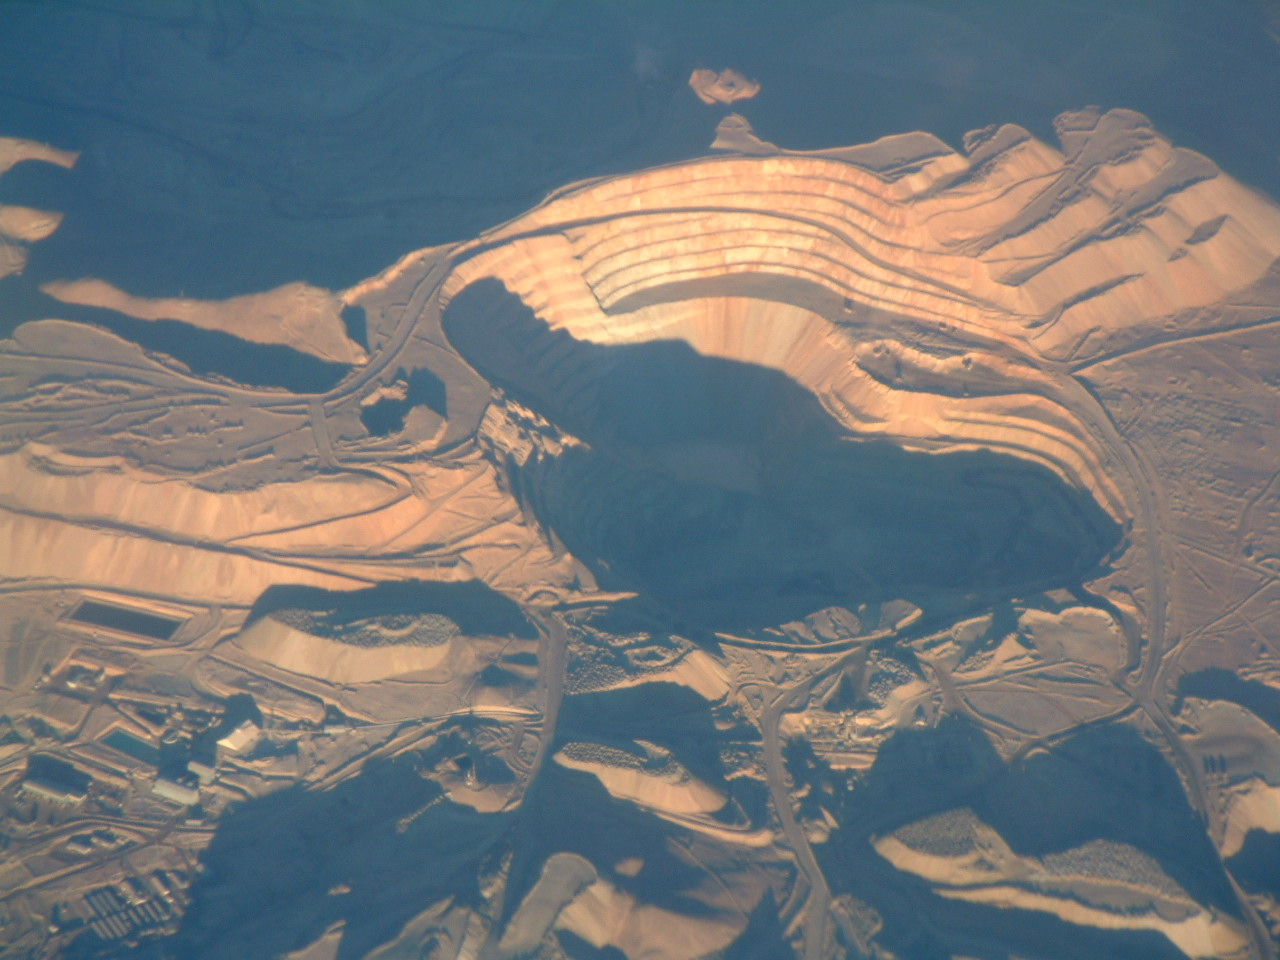
\includegraphics[width=0.82\textwidth]{../presentacion_latex/imagenes/chuquicamata.jpg}
\end{center}

\begin{abstract}
Este informe presenta el trabajo realizado con un archivo oficial de COCHILCO sobre producción mensual de cobre de mina por empresa/faena. El archivo original no venía listo para analizar: tenía títulos, filas de resumen, notas y meses sin información efectiva. Por eso, primero se ordenó la base y luego se revisaron sus principales patrones. El documento explica qué datos se usaron, qué problemas aparecieron, qué decisiones de limpieza se tomaron y qué resultados entregó el análisis exploratorio.
\end{abstract}

\tableofcontents
\newpage

\section{Introducción}

La minería del cobre tiene un peso evidente en la economía chilena. Por eso, trabajar con datos de producción minera permite mirar un tema relevante y, al mismo tiempo, practicar limpieza y análisis exploratorio con una base real. En este caso se usó un archivo oficial de la Comisión Chilena del Cobre (COCHILCO), específicamente la producción mensual de cobre de mina por empresa/faena.

El foco no estuvo solo en graficar, sino también en dejar claro qué se hizo con los datos antes de analizarlos. El Excel original estaba pensado para consulta humana, no necesariamente para ser leído directamente por Python. Esa diferencia explica buena parte del trabajo de preprocesamiento.

\section{Fuente y descripción general del dataset}

El archivo utilizado corresponde a \textit{Producción de Cobre Mina por Empresa Mensual}, publicado por COCHILCO. La unidad de medida es miles de toneladas métricas de cobre fino. El Excel trae la información mensual por empresa/faena, pero también incluye elementos de presentación, como títulos, subtítulos, notas, resúmenes anuales y fuente. Esos elementos son útiles al leer la planilla, pero complican el análisis automatizado.

La Tabla \ref{tab:resumen-general} resume los principales atributos del dataset después de la limpieza.

\begin{table}[H]
\centering
\caption{Resumen general del dataset limpio}
\label{tab:resumen-general}
\begin{tabular}{lp{0.62\textwidth}}
\toprule
Aspecto & Valor \\
\midrule
Fuente & COCHILCO \\
Archivo original & Producción de Cobre Mina por Empresa Mensual \\
Unidad & Miles de toneladas métricas de cobre fino \\
Período limpio & 2014-01-01 a 2026-03-01 \\
Observaciones formato ancho & 147 \\
Columnas formato ancho & 44 \\
Registros formato largo & 5694 \\
Empresas/faenas con producción positiva & 41 \\
Valores faltantes en dataset limpio ancho & 0 \\
Duplicados exactos en dataset limpio ancho & 0 \\
\bottomrule
\end{tabular}

\end{table}

El dataset limpio se dejó en dos versiones. La primera conserva el formato ancho, parecido al Excel original: una fila por mes y una columna por empresa/faena o total agregado. La segunda es una versión en formato largo: cada fila corresponde a una fecha y una empresa/faena con producción positiva. Esta segunda forma no cambia los datos de origen; solo los reorganiza para hacer más simple la comparación entre faenas.

\section{Variables del dataset}

\subsection{Estructura general}

La variable temporal principal es \code{fecha}, que identifica el mes observado. El resto de columnas corresponde a producción mensual de cobre de mina, medida en miles de toneladas métricas de cobre fino. Algunas columnas son faenas específicas, como \code{escondida}, \code{collahuasi} o \code{los_pelambres}; otras son agregados, como \code{total_codelco} y \code{total_chile}.

Como el archivo original tiene una columna por faena, está en formato ancho. Ese formato es cómodo para mirar una planilla, pero no siempre es el más práctico para agrupar por faena. Por eso se creó también una versión larga con estas variables:

\begin{itemize}[itemsep=0.2em]
    \item \code{fecha}: mes de observación.
    \item \code{empresa_faena}: nombre limpio de la empresa o faena.
    \item \code{produccion_miles_tm_cobre_fino}: producción mensual.
    \item \code{anio}: año de la observación.
    \item \code{mes}: mes numérico de la observación.
\end{itemize}

\subsection{Diccionario de variables}

La Tabla \ref{tab:diccionario-variables} presenta todas las variables del dataset limpio en formato ancho. Este diccionario permite entender qué representa cada columna y diferencia entre fecha, faenas individuales y totales agregados.

\begin{center}
\captionof{table}{Diccionario de variables del dataset limpio}
\label{tab:diccionario-variables}
\begin{longtable}{p{0.23\textwidth}p{0.16\textwidth}p{0.52\textwidth}}
\toprule
Variable limpia & Tipo & Descripción \\
\midrule
\endfirsthead
\toprule
Variable limpia & Tipo & Descripción \\
\midrule
\endhead
fecha & Fecha & Mes de referencia de la observación. \\
chuqui\_y\_r\_tomic & Empresa/faena & Producción mensual de cobre de mina reportada para chuqui y r tomic. \\
chuquicamata & Empresa/faena & Producción mensual de cobre de mina reportada para chuquicamata. \\
radomiro\_tomic & Empresa/faena & Producción mensual de cobre de mina reportada para radomiro tomic. \\
ministro\_hales & Empresa/faena & Producción mensual de cobre de mina reportada para ministro hales. \\
salvador & Empresa/faena & Producción mensual de cobre de mina reportada para salvador. \\
andina & Empresa/faena & Producción mensual de cobre de mina reportada para andina. \\
el\_teniente & Empresa/faena & Producción mensual de cobre de mina reportada para el teniente. \\
gabriela\_mistral & Empresa/faena & Producción mensual de cobre de mina reportada para gabriela mistral. \\
total\_codelco & Total agregado & Producción mensual agregada de faenas Codelco incluidas en el archivo. \\
escondida & Empresa/faena & Producción mensual de cobre de mina reportada para escondida. \\
spence & Empresa/faena & Producción mensual de cobre de mina reportada para spence. \\
cerro\_colorado & Empresa/faena & Producción mensual de cobre de mina reportada para cerro colorado. \\
lomas\_bayas & Empresa/faena & Producción mensual de cobre de mina reportada para lomas bayas. \\
collahuasi & Empresa/faena & Producción mensual de cobre de mina reportada para collahuasi. \\
los\_bronces & Empresa/faena & Producción mensual de cobre de mina reportada para los bronces. \\
el\_soldado & Empresa/faena & Producción mensual de cobre de mina reportada para el soldado. \\
angloamerican\_sur & Empresa/faena & Producción mensual de cobre de mina reportada para angloamerican sur. \\
el\_abra & Empresa/faena & Producción mensual de cobre de mina reportada para el abra. \\
candelaria & Empresa/faena & Producción mensual de cobre de mina reportada para candelaria. \\
caserones & Empresa/faena & Producción mensual de cobre de mina reportada para caserones. \\
ojos\_del\_salado & Empresa/faena & Producción mensual de cobre de mina reportada para ojos del salado. \\
mantos\_blancos & Empresa/faena & Producción mensual de cobre de mina reportada para mantos blancos. \\
mantoverde & Empresa/faena & Producción mensual de cobre de mina reportada para mantoverde. \\
capstone\_copper & Empresa/faena & Producción mensual de cobre de mina reportada para capstone copper. \\
los\_pelambres & Empresa/faena & Producción mensual de cobre de mina reportada para los pelambres. \\
zaldivar & Empresa/faena & Producción mensual de cobre de mina reportada para zaldivar. \\
centinela\_sulfuros & Empresa/faena & Producción mensual de cobre de mina reportada para centinela sulfuros. \\
centinela\_oxidos & Empresa/faena & Producción mensual de cobre de mina reportada para centinela oxidos. \\
antucoya & Empresa/faena & Producción mensual de cobre de mina reportada para antucoya. \\
quebrada\_blanca & Empresa/faena & Producción mensual de cobre de mina reportada para quebrada blanca. \\
andacollo & Empresa/faena & Producción mensual de cobre de mina reportada para andacollo. \\
michilla & Empresa/faena & Producción mensual de cobre de mina reportada para michilla. \\
haldeman & Empresa/faena & Producción mensual de cobre de mina reportada para haldeman. \\
sierra\_gorda & Empresa/faena & Producción mensual de cobre de mina reportada para sierra gorda. \\
atacama\_kozan & Empresa/faena & Producción mensual de cobre de mina reportada para atacama kozan. \\
tres\_valles & Empresa/faena & Producción mensual de cobre de mina reportada para tres valles. \\
franke & Empresa/faena & Producción mensual de cobre de mina reportada para franke. \\
altos\_de\_punitaqui & Empresa/faena & Producción mensual de cobre de mina reportada para altos de punitaqui. \\
cerro\_negro & Empresa/faena & Producción mensual de cobre de mina reportada para cerro negro. \\
pampa\_camarones & Empresa/faena & Producción mensual de cobre de mina reportada para pampa camarones. \\
enami\_plantas & Empresa/faena & Producción mensual de cobre de mina reportada para enami plantas. \\
otros & Empresa/faena & Producción mensual agrupada en la categoría Otros. \\
total\_chile & Total agregado & Producción total mensual de cobre de mina en Chile. \\
\bottomrule
\end{longtable}

\end{center}

\section{Problemas detectados en el archivo original}

El archivo de COCHILCO no venía directamente como una base de datos lista para análisis. Era una planilla de publicación. Por eso, antes de calcular estadísticas, fue necesario separar los datos mensuales de los elementos de formato.

Los principales problemas detectados fueron:

\begin{itemize}[itemsep=0.2em]
    \item \textbf{Encabezados institucionales}: las primeras filas contenían títulos y nombres institucionales, no observaciones.
    \item \textbf{Fila de encabezado desplazada}: los nombres reales de las columnas se encontraban en una fila interna del Excel, por lo que se usó \texttt{header=6}.
    \item \textbf{Filas anuales}: el archivo mezclaba meses con resúmenes anuales, lo que podía distorsionar el análisis mensual.
    \item \textbf{Nota de fuente}: al final del archivo había una fila textual con la fuente del dato.
    \item \textbf{Meses sin dato informado}: algunos meses futuros aparecían con producción total igual a cero y múltiples valores faltantes.
    \item \textbf{Nombres de columnas no estandarizados}: existían espacios, mayúsculas, acentos y paréntesis.
    \item \textbf{Formato ancho}: cada empresa/faena estaba en una columna distinta, lo que dificulta ciertas comparaciones por grupo.
\end{itemize}

\section{Proceso de limpieza}

La limpieza buscó dejar una base mensual consistente y reproducible. La Tabla \ref{tab:flujo-limpieza} muestra cómo se pasó desde el Excel original hasta los archivos limpios.

\begin{table}[H]
\centering
\caption{Flujo de limpieza aplicado al dataset}
\label{tab:flujo-limpieza}
\begin{tabular}{lrrp{0.43\textwidth}}
\toprule
Etapa & Filas & Columnas & Criterio \\
\midrule
Archivo original leído desde Excel & 171 & 44 & Incluye títulos, filas anuales y nota de fuente. \\
Filas no vacías después de lectura & 170 & 44 & Se eliminan filas totalmente vacías. \\
Filas mensuales identificadas & 156 & 44 & Se conservan registros cuyo campo fecha es mensual. \\
Meses con producción nacional informada & 147 & 44 & Se filtra total\_chile mayor que cero. \\
Dataset limpio en formato largo & 5694 & 5 & Una fila por fecha y empresa/faena con producción positiva. \\
\bottomrule
\end{tabular}

\end{table}

Las principales acciones de limpieza fueron:

\begin{enumerate}[itemsep=0.2em]
    \item \textbf{Lectura correcta del encabezado}: se cargó el Excel con \texttt{header=6}, porque ahí estaban los nombres reales de las columnas.
    \item \textbf{Eliminación de filas vacías}: se descartaron filas completamente vacías.
    \item \textbf{Filtrado de observaciones mensuales}: se conservaron solo filas cuya primera columna correspondía a una fecha mensual.
    \item \textbf{Estandarización de nombres}: se transformaron los nombres a minúsculas, sin espacios, sin acentos y con guiones bajos.
    \item \textbf{Conversión de tipos}: la fecha se convirtió a \texttt{datetime} y las columnas productivas a valores numéricos.
    \item \textbf{Eliminación de meses sin producción informada}: se filtraron filas con \code{total_chile} igual a cero.
    \item \textbf{Transformación a formato largo}: se creó un dataset con una fila por mes y empresa/faena con producción positiva.
\end{enumerate}

\subsection{Valores faltantes}

En el archivo mensual antes del filtro final existían valores faltantes, principalmente asociados a meses futuros o faenas sin registro en determinadas fechas. La Tabla \ref{tab:faltantes-original} muestra las variables con mayor cantidad de faltantes en la versión mensual intermedia.

\begin{table}[H]
\centering
\caption{Principales valores faltantes antes del filtro final}
\label{tab:faltantes-original}
\begin{tabular}{lrr}
\toprule
Variable & Faltantes & \textbackslash\{\}\% \\
\midrule
chuquicamata & 9 & 5,77 \\
mantoverde & 9 & 5,77 \\
los\_pelambres & 9 & 5,77 \\
zaldivar & 9 & 5,77 \\
centinela\_sulfuros & 9 & 5,77 \\
centinela\_oxidos & 9 & 5,77 \\
antucoya & 9 & 5,77 \\
quebrada\_blanca & 9 & 5,77 \\
andacollo & 9 & 5,77 \\
michilla & 9 & 5,77 \\
haldeman & 9 & 5,77 \\
sierra\_gorda & 9 & 5,77 \\
\bottomrule
\end{tabular}

\end{table}

Después de la limpieza final, el dataset ancho usado en el análisis quedó sin valores faltantes y sin duplicados exactos. Por eso no fue necesario imputar datos para las estadísticas principales.

\section{Análisis exploratorio}

\subsection{Estadísticas descriptivas}

La Tabla \ref{tab:estadisticas-descriptivas} resume las principales estadísticas de variables seleccionadas. Se eligieron \code{total_chile}, \code{total_codelco} y algunas faenas relevantes porque permiten comparar la producción nacional con productores de gran escala.

\begin{table}[H]
\centering
\caption{Estadísticas descriptivas de variables seleccionadas}
\label{tab:estadisticas-descriptivas}
\begin{tabular}{lrrrrr}
\toprule
Variable & Media & Desv. est. & Mín. & Mediana & Máx. \\
\midrule
total\_chile & 464,52 & 34,54 & 370,84 & 465,99 & 563,60 \\
total\_codelco & 129,60 & 20,11 & 79,85 & 132,35 & 177,67 \\
escondida & 95,00 & 17,22 & 0,00 & 95,50 & 133,61 \\
collahuasi & 44,47 & 7,64 & 16,98 & 44,49 & 60,32 \\
los\_pelambres & 28,98 & 4,58 & 14,00 & 29,40 & 38,10 \\
el\_teniente & 35,22 & 6,77 & 11,53 & 36,57 & 52,43 \\
\bottomrule
\end{tabular}

\end{table}

La producción total mensual de Chile tiene una media de 464,52 miles de toneladas métricas de cobre fino y una mediana de 465,99. Como ambos valores son cercanos, el total nacional no parece tener un sesgo muy marcado. Aun así, hay meses bastante bajos y otros bastante altos, por lo que más adelante se revisan como posibles valores atípicos.

En las faenas individuales, Escondida destaca con una media mensual cercana a 95,00. Esto la deja por sobre las otras faenas seleccionadas y confirma su peso dentro de la producción minera chilena.

\subsection{Histogramas}

Los histogramas se usaron porque la producción mensual es una variable numérica continua. En este caso ayudan a ver dónde se concentran los meses y si aparecen valores alejados del comportamiento habitual.

\begin{figure}[H]
\centering
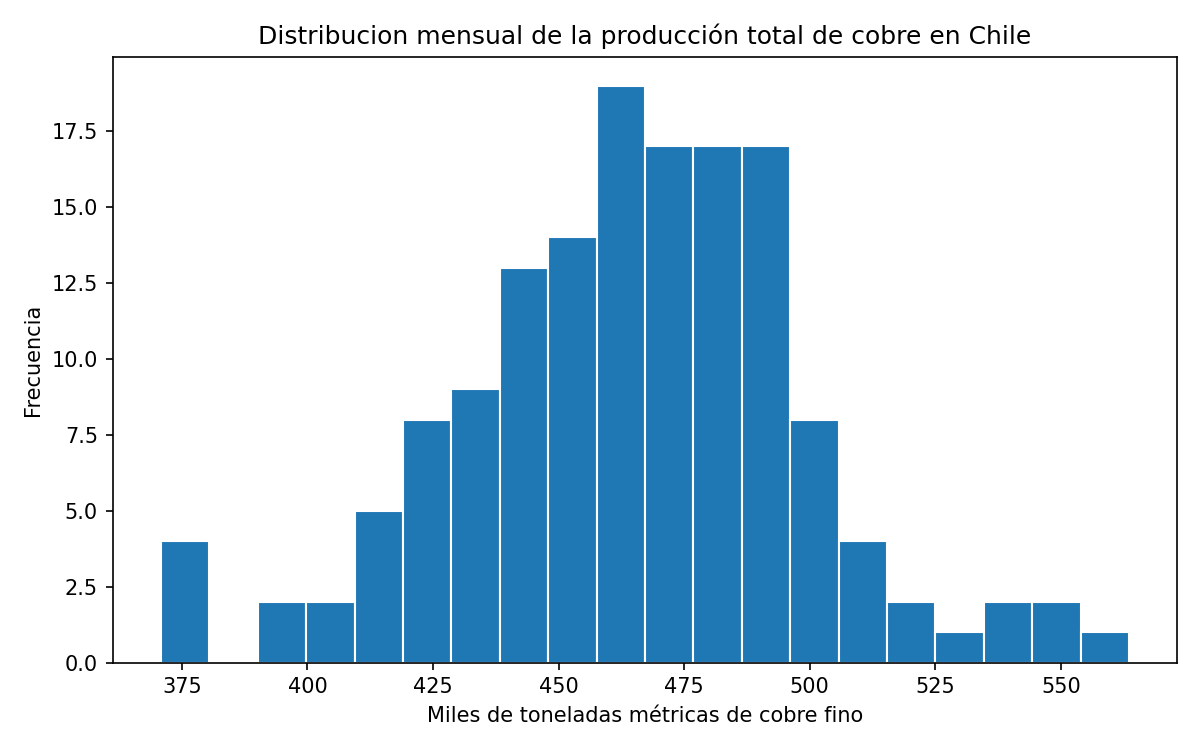
\includegraphics[width=0.82\textwidth]{figuras/hist_total_chile.png}
\caption{Histograma de la producción total mensual de cobre en Chile}
\label{fig:hist-total-chile}
\end{figure}

La Figura \ref{fig:hist-total-chile} muestra que la producción nacional se concentra principalmente entre 445 y 487 miles de toneladas métricas. También aparecen algunos valores en los extremos, que corresponden a meses de producción inusualmente baja o alta.

\begin{figure}[H]
\centering
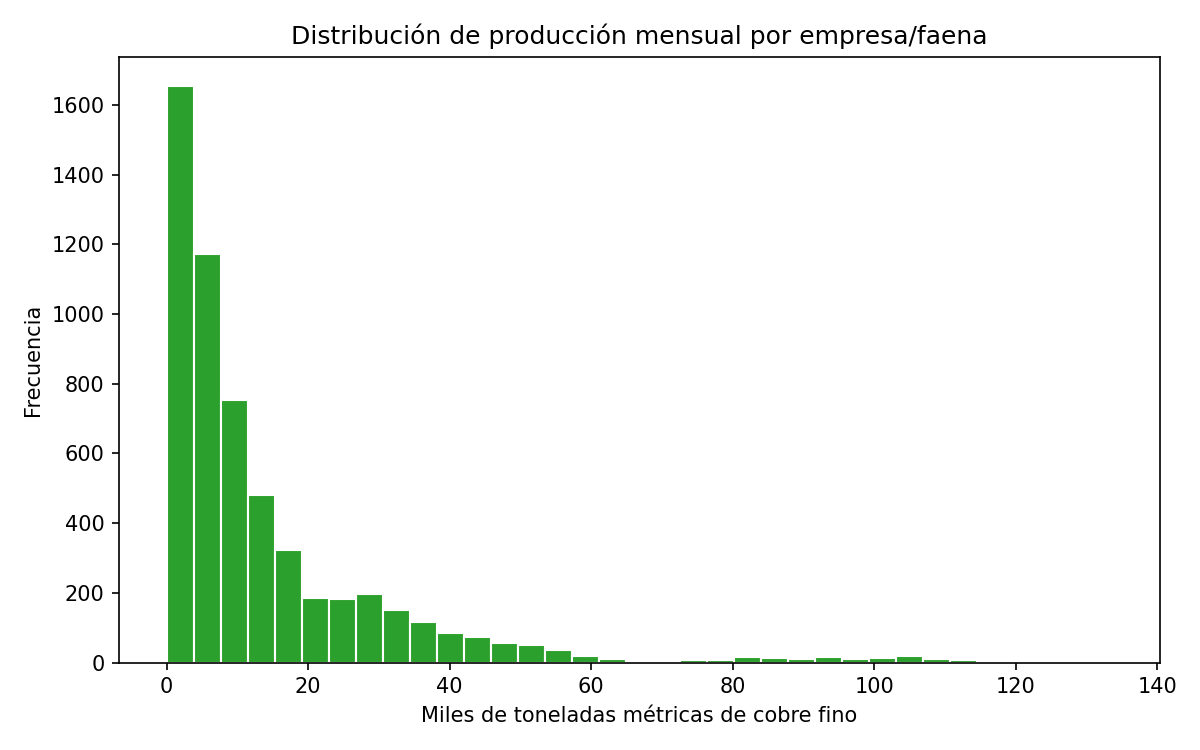
\includegraphics[width=0.82\textwidth]{figuras/hist_empresas_faenas.png}
\caption{Histograma de producción mensual por empresa/faena}
\label{fig:hist-faenas}
\end{figure}

La Figura \ref{fig:hist-faenas} es mucho más asimétrica. La mayoría de las observaciones está en producciones bajas o medias, mientras que pocas faenas llegan a niveles muy altos. Esto calza con la estructura del sector: conviven operaciones muy grandes con otras de menor escala.

\subsection{Principales empresas/faenas}

La Tabla \ref{tab:top-faenas} presenta las diez empresas/faenas con mayor producción promedio mensual considerando solo meses con producción positiva en el dataset largo.

\begin{table}[H]
\centering
\caption{Empresas/faenas con mayor producción promedio mensual en meses con producción positiva}
\label{tab:top-faenas}
\begin{tabular}{lrrrrr}
\toprule
Empresa/faena & Meses positivos & Media positiva & Total & Mín. & Máx. \\
\midrule
escondida & 146 & 95,65 & 13964,37 & 20,00 & 133,61 \\
chuqui\_y\_r\_tomic & 147 & 51,31 & 7542,80 & 32,26 & 80,03 \\
collahuasi & 147 & 44,47 & 6536,83 & 16,98 & 60,32 \\
el\_teniente & 147 & 35,22 & 5177,00 & 11,53 & 52,43 \\
los\_pelambres & 147 & 28,98 & 4260,71 & 14,00 & 38,10 \\
angloamerican\_sur & 147 & 28,45 & 4181,60 & 15,56 & 43,34 \\
chuquicamata & 147 & 26,01 & 3823,20 & 11,36 & 54,04 \\
radomiro\_tomic & 147 & 25,30 & 3719,60 & 14,15 & 35,32 \\
los\_bronces & 147 & 24,83 & 3650,61 & 11,33 & 40,19 \\
spence & 147 & 16,92 & 2486,77 & 6,10 & 30,11 \\
\bottomrule
\end{tabular}

\end{table}

Escondida aparece como la faena con mayor producción promedio mensual en meses con producción positiva. Luego vienen Chuqui y R. Tomic, Collahuasi, El Teniente y Los Pelambres. La lectura principal es que la producción está concentrada: pocas operaciones grandes explican una parte importante del volumen total.

Hay que distinguir este promedio del promedio de Escondida en la Tabla \ref{tab:estadisticas-descriptivas}. Allí la media es 95,00 porque se calcula sobre los 147 meses del formato ancho e incluye marzo de 2017, mes en que Escondida registra producción 0. En cambio, la Tabla \ref{tab:top-faenas} usa el dataset largo filtrado a producción positiva, por lo que Escondida queda con 146 meses y una media de 95,65. La diferencia no es una contradicción: son dos criterios de cálculo distintos.

\section{Correlaciones y diagramas de dispersión}

\subsection{Matriz de correlaciones}

La correlación mide qué tan juntas se mueven dos variables en términos lineales. Va de -1 a 1: valores cercanos a 1 indican relación positiva fuerte; valores cercanos a -1 indican relación negativa fuerte; valores cercanos a 0 indican poca relación lineal.

\begin{table}[H]
\centering
\caption{Matriz de correlaciones entre variables seleccionadas}
\label{tab:correlaciones}
\resizebox{\textwidth}{!}{\begin{tabular}{lrrrrrr}
\toprule
Variable & total\_chile & total\_codelco & escondida & collahuasi & los\_pelambres & el\_teniente \\
\midrule
total\_chile & 1,00 & 0,77 & 0,44 & 0,30 & 0,57 & 0,59 \\
total\_codelco & 0,77 & 1,00 & -0,09 & 0,22 & 0,52 & 0,80 \\
escondida & 0,44 & -0,09 & 1,00 & -0,14 & -0,04 & -0,10 \\
collahuasi & 0,30 & 0,22 & -0,14 & 1,00 & 0,14 & 0,22 \\
los\_pelambres & 0,57 & 0,52 & -0,04 & 0,14 & 1,00 & 0,41 \\
el\_teniente & 0,59 & 0,80 & -0,10 & 0,22 & 0,41 & 1,00 \\
\bottomrule
\end{tabular}
}
\end{table}

La correlación entre \code{total_codelco} y \code{total_chile} es 0,77. Es una relación positiva alta: cuando aumenta la producción agregada de Codelco, el total nacional tiende a moverse en la misma dirección. Dado el tamaño de Codelco dentro del sector, este resultado es razonable.

La correlación entre \code{escondida} y \code{total_chile} es 0,44. Escondida es muy importante como faena individual, pero el total nacional no depende solo de ella. Por eso la relación existe, aunque es más moderada.

La correlación entre \code{total_codelco} y \code{el_teniente} es 0,80. Tiene sentido, porque El Teniente forma parte de Codelco y sus variaciones se reflejan en el agregado de la empresa.

\subsection{Correlación de cada variable con el total nacional}

Además de la matriz reducida, se calculó la correlación de cada variable productiva con \code{total_chile}. La Tabla \ref{tab:correlaciones-total-chile} permite identificar qué faenas o agregados se mueven más cerca del total nacional y cuáles tienen una relación más débil.

\begin{center}
\captionof{table}{Correlación de cada variable con la producción total de Chile}
\label{tab:correlaciones-total-chile}
\begin{longtable}{p{0.31\textwidth}rrp{0.18\textwidth}}
\toprule
Variable & Correlación con total\_chile & Sentido & Intensidad \\
\midrule
\endfirsthead
\toprule
Variable & Correlación con total\_chile & Sentido & Intensidad \\
\midrule
\endhead
total\_codelco & 0,77 & Positiva & Alta \\
chuqui\_y\_r\_tomic & 0,75 & Positiva & Alta \\
chuquicamata & 0,71 & Positiva & Alta \\
el\_teniente & 0,59 & Positiva & Media \\
los\_pelambres & 0,57 & Positiva & Media \\
salvador & 0,52 & Positiva & Media \\
zaldivar & 0,47 & Positiva & Media \\
ojos\_del\_salado & 0,44 & Positiva & Media \\
escondida & 0,44 & Positiva & Media \\
ministro\_hales & 0,39 & Positiva & Baja \\
angloamerican\_sur & 0,39 & Positiva & Baja \\
gabriela\_mistral & 0,39 & Positiva & Baja \\
tres\_valles & 0,39 & Positiva & Baja \\
los\_bronces & 0,37 & Positiva & Baja \\
centinela\_sulfuros & 0,36 & Positiva & Baja \\
andacollo & 0,35 & Positiva & Baja \\
franke & 0,34 & Positiva & Baja \\
andina & 0,33 & Positiva & Baja \\
radomiro\_tomic & 0,31 & Positiva & Baja \\
collahuasi & 0,30 & Positiva & Baja \\
otros & 0,30 & Positiva & Baja \\
cerro\_colorado & 0,27 & Positiva & Baja \\
lomas\_bayas & 0,26 & Positiva & Baja \\
centinela\_oxidos & 0,25 & Positiva & Baja \\
altos\_de\_punitaqui & 0,24 & Positiva & Baja \\
el\_soldado & 0,23 & Positiva & Baja \\
haldeman & 0,21 & Positiva & Baja \\
el\_abra & 0,20 & Positiva & Baja \\
cerro\_negro & 0,18 & Positiva & Baja \\
enami\_plantas & 0,14 & Positiva & Baja \\
michilla & 0,13 & Positiva & Baja \\
atacama\_kozan & 0,13 & Positiva & Baja \\
mantos\_blancos & 0,10 & Positiva & Baja \\
candelaria & 0,09 & Positiva & Baja \\
capstone\_copper & 0,07 & Positiva & Baja \\
mantoverde & 0,05 & Positiva & Baja \\
caserones & -0,01 & Negativa & Baja \\
pampa\_camarones & -0,06 & Negativa & Baja \\
quebrada\_blanca & -0,11 & Negativa & Baja \\
sierra\_gorda & -0,11 & Negativa & Baja \\
antucoya & -0,13 & Negativa & Baja \\
spence & -0,14 & Negativa & Baja \\
\bottomrule
\end{longtable}

\end{center}

Esta tabla no debe leerse como causalidad. Una correlación alta solo indica que dos series se mueven juntas de forma lineal. En este caso, las correlaciones más altas aparecen en operaciones o agregados que tienen más peso productivo o que se parecen más al ciclo mensual nacional.

\subsection{Diagramas de dispersión}

Los diagramas de dispersión se usaron para mirar visualmente las relaciones entre variables productivas. Sirven para ver si la nube de puntos sugiere una relación positiva, negativa o si no hay un patrón claro.

\begin{figure}[H]
\centering
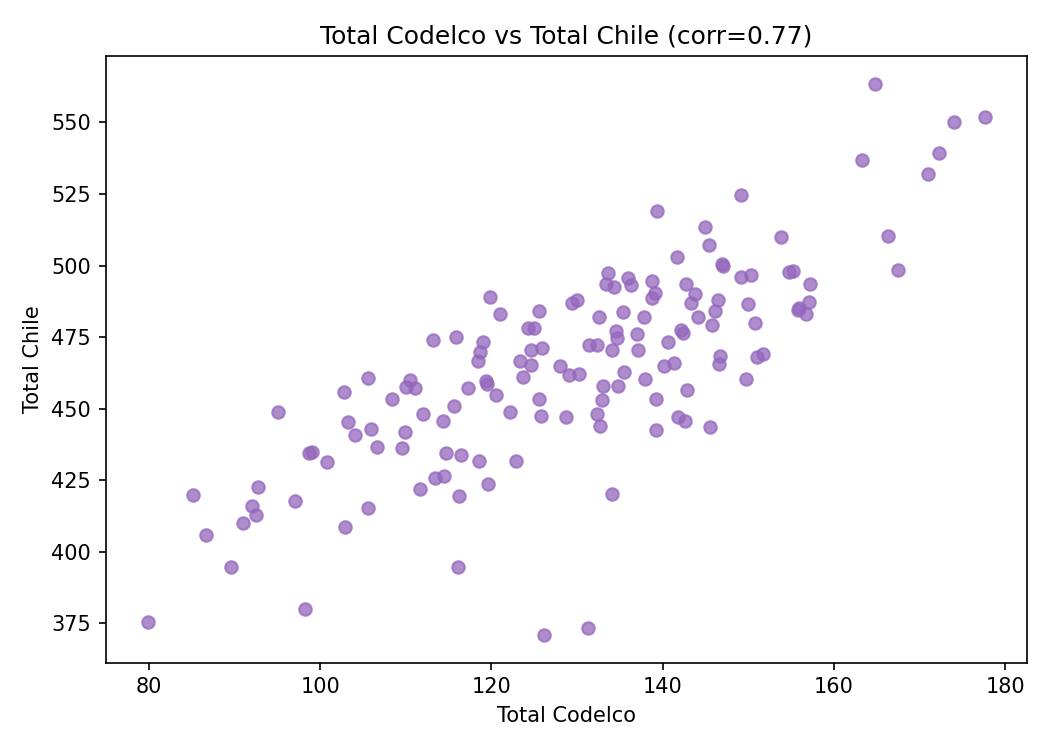
\includegraphics[width=0.78\textwidth]{figuras/scatter_codelco_total_chile.png}
\caption{Relación entre producción de Codelco y producción total de Chile}
\label{fig:scatter-codelco}
\end{figure}

En la Figura \ref{fig:scatter-codelco} la nube de puntos sube de izquierda a derecha. Eso respalda visualmente la correlación positiva entre Codelco y el total nacional.

\begin{figure}[H]
\centering
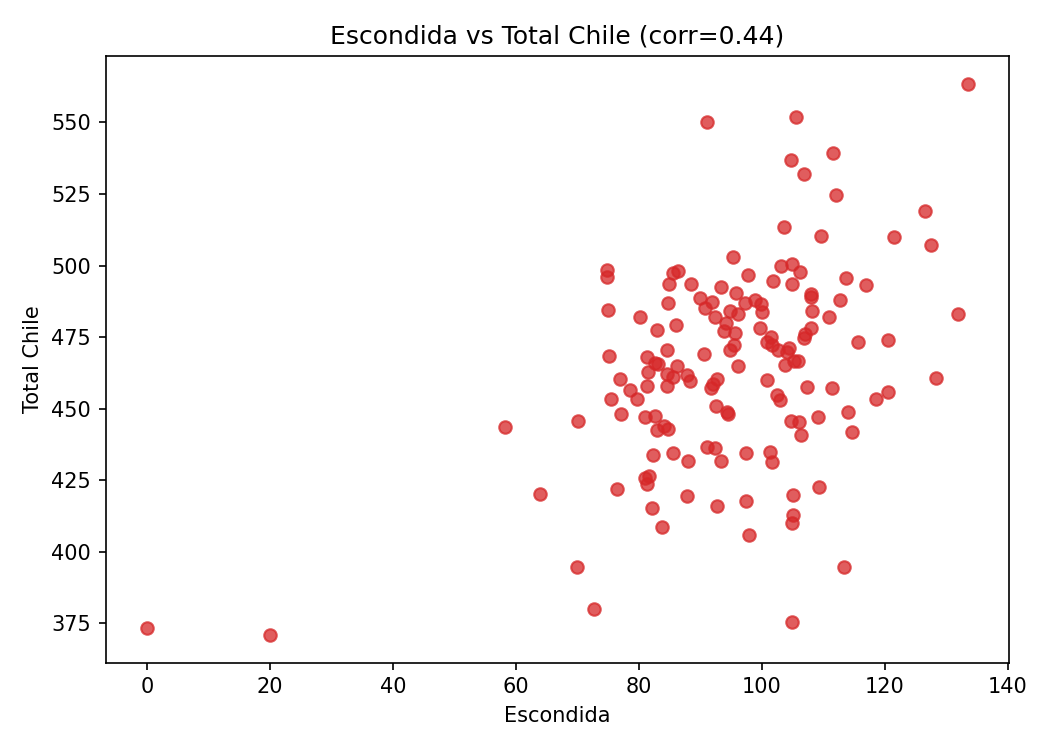
\includegraphics[width=0.78\textwidth]{figuras/scatter_escondida_total_chile.png}
\caption{Relación entre producción de Escondida y producción total de Chile}
\label{fig:scatter-escondida}
\end{figure}

En la Figura \ref{fig:scatter-escondida} también se ve una relación positiva, pero con más dispersión. Escondida pesa bastante, aunque el total nacional responde a una combinación más amplia de productores.

\section{Outliers, asimetría y concentración}

\subsection{Asimetría y curtosis}

La asimetría indica si una distribución se carga hacia un lado. Si es positiva, la cola va hacia valores altos; si es negativa, hacia valores bajos. La curtosis ayuda a ver si la distribución tiene valores muy concentrados o colas más marcadas.

\begin{table}[H]
\centering
\caption{Asimetría y curtosis de variables seleccionadas}
\label{tab:asimetria}
\begin{tabular}{lrr}
\toprule
Variable & Asimetría & Curtosis \\
\midrule
total\_chile & -0,12 & 0,69 \\
total\_codelco & -0,13 & -0,29 \\
escondida & -1,53 & 7,48 \\
collahuasi & -0,36 & 0,48 \\
los\_pelambres & -0,76 & 0,91 \\
el\_teniente & -0,72 & 0,57 \\
\bottomrule
\end{tabular}

\end{table}

El total nacional tiene una asimetría levemente negativa, por lo que no muestra un sesgo extremo. Escondida, en cambio, presenta una asimetría negativa más marcada y una curtosis alta. Eso refleja meses que se alejan bastante de su comportamiento típico.

\subsection{Detección de outliers}

Para identificar outliers en \code{total_chile} se utilizó el rango intercuartil (IQR). El criterio considera como potenciales outliers los valores inferiores a:

\[
Q_1 - 1{,}5 \times IQR
\]

y superiores a:

\[
Q_3 + 1{,}5 \times IQR
\]

La Tabla \ref{tab:outliers} muestra los meses detectados como valores atípicos para la producción total nacional.

\begin{table}[H]
\centering
\caption{Meses atípicos detectados para la producción total de Chile}
\label{tab:outliers}
\begin{tabular}{lrrr}
\toprule
Mes & Total Chile & Total Codelco & Escondida \\
\midrule
2017-02 & 370,84 & 126,17 & 20,00 \\
2017-03 & 373,13 & 131,26 & 0,00 \\
2018-12 & 550,09 & 174,03 & 91,10 \\
2019-12 & 551,75 & 177,67 & 105,66 \\
2023-02 & 379,96 & 98,23 & 72,70 \\
2024-12 & 563,60 & 164,78 & 133,61 \\
2026-02 & 375,39 & 79,85 & 105,02 \\
\bottomrule
\end{tabular}

\end{table}

Estos valores no se eliminaron automáticamente. En minería, un mes atípico puede reflejar algo real: mantenciones, paralizaciones, variaciones operacionales, conflictos laborales, cambios de planificación o cierres de período. Por eso se trataron como observaciones que conviene mirar con contexto, no como errores que haya que borrar de inmediato.

\section{Resultados principales}

Los resultados que considero más relevantes son los siguientes:

\begin{itemize}[itemsep=0.25em]
    \item El dataset limpio cubre el período enero de 2014 a marzo de 2026.
    \item La producción total mensual promedio de Chile fue de 464,52 miles de toneladas métricas de cobre fino.
    \item Escondida fue la faena con mayor producción promedio mensual positiva entre las operaciones individuales.
    \item Codelco tiene una correlación alta con la producción total nacional, lo que refleja su importancia agregada.
    \item La distribución por empresa/faena es asimétrica: muchas faenas tienen producciones bajas o medias y pocas operaciones concentran volúmenes altos.
    \item Se detectaron meses atípicos en el total nacional, pero se conservaron porque pueden tener significado económico u operacional.
    \item El paso de formato ancho a formato largo mejora la capacidad de análisis por empresa, año, mes y faena.
\end{itemize}

\section{Conclusiones}

El archivo de COCHILCO trae información valiosa, pero no viene listo para analizar directamente. La principal dificultad no fue la falta de datos, sino la forma del Excel: títulos, filas anuales, notas y meses sin información productiva mezclados con observaciones mensuales.

Después de la limpieza, el dataset queda en condiciones de analizarse. La producción nacional de cobre se ve relativamente estable, pero aparecen meses puntuales de producción muy baja o muy alta. Esos meses no deberían eliminarse sin revisar el contexto, porque pueden corresponder a hechos reales del sector.

La comparación por empresas/faenas muestra concentración productiva. Escondida destaca como faena individual, mientras que Codelco, como agregado, se relaciona más fuertemente con el total nacional. Esa diferencia ayuda a separar el peso de una operación puntual del peso de un conjunto de faenas.

En resumen, la limpieza permitió pasar de una planilla institucional a una base más ordenada. Con esa base se pudieron revisar estadísticas descriptivas, histogramas, diagramas de dispersión, valores faltantes, outliers y medidas de asimetría y concentración.

\section{Archivos generados}

Como resultado del trabajo se generaron los siguientes archivos principales:

\begin{itemize}[itemsep=0.2em]
    \item \code{produccion_cobre_mensual_limpio_ancho.csv}: dataset mensual limpio en formato ancho.
    \item \code{produccion_cobre_mensual_limpio_largo.csv}: dataset limpio en formato largo.
    \item \code{resumen_produccion_por_empresa.csv}: resumen estadístico por empresa/faena.
    \item \code{notebooks/tarea_1_limpieza_datos.ipynb}: notebook ejecutado con código, resultados y gráficos.
    \item \code{main.pdf}: presentación Beamer de la tarea.
    \item \code{informe_limpieza_datos_mineria_chilena.pdf}: este informe.
\end{itemize}

\section{Fuente}

La fuente principal de datos es COCHILCO:

\begin{itemize}
    \item \url{https://www.cochilco.cl/web/historico-produccion-de-cobre-y-molibdeno/}
\end{itemize}

\end{document}
